% !TeX program = pdflatex
% CoderUJB presentation: 32 slides, including cover, contents, six section pages and all 24 content slides.
% Derived from the supplied 24-slide French PPTX.
% Visual reference supplied by the user: sildeS2Groupe1.pdf.
% Its native Beamer settings are available in rapportS2_beamer.tex.
% Only layout settings are reused; the source project's content and identity are not imported.
\documentclass[aspectratio=169,usepdftitle=false]{beamer}
\mode<presentation>
{
  \usetheme{default}
  \usecolortheme{default}
  \usefonttheme{default}
  \setbeamertemplate{navigation symbols}{}
  \setbeamertemplate{caption}[numbered]
  \setbeamertemplate{footline}{%
    \leavevmode%
    \hbox{%
      \begin{beamercolorbox}[wd=\paperwidth,ht=2.6ex,dp=1.2ex,rightskip=1.2em]{author in head/foot}%
        \hfill\usebeamerfont{author in head/foot}\insertframenumber
      \end{beamercolorbox}%
    }%
  }
}
\usepackage[french]{babel}
\usepackage[utf8]{inputenc}
\usepackage[T1]{fontenc}
\usepackage{lmodern}
\usepackage{amsmath}
\usepackage{amssymb}
\usepackage{booktabs}
\usepackage{array}
\usepackage{ragged2e}
\usepackage{tikz}

% Give slide headings the same left margin as the body and extra top space.
\setbeamertemplate{frametitle}{%
  \nointerlineskip
  \vspace*{0.70cm}%
  \begin{beamercolorbox}[wd=\paperwidth,leftskip=1cm,rightskip=1cm,sep=0pt]{frametitle}
    \usebeamerfont{frametitle}\strut\insertframetitle\strut\par
  \end{beamercolorbox}%
  \vspace*{0.12cm}%
}

\AtBeginEnvironment{frame}{\justifying}
\AtBeginEnvironment{block}{\justifying}
\AtBeginEnvironment{alertblock}{\justifying}
\AtBeginEnvironment{exampleblock}{\justifying}
\addtobeamertemplate{itemize/enumerate body begin}{\justifying}{}
\addtobeamertemplate{itemize/enumerate subbody begin}{\justifying}{}
\addtobeamertemplate{itemize/enumerate subsubbody begin}{\justifying}{}
\setbeameroption{hide notes}
\hypersetup{
  pdftitle={CoderUJB -- Presentation},
  pdfauthor={Wei WEI, Hao QIAN, Jianye SHI, Xiang BIAN, Zijie Fang, Yupan Huang},
  pdfsubject={Presentation de l'article CoderUJB, ISSTA 2024},
  pdfkeywords={CoderUJB, Java, LLM, benchmark, ISSTA 2024}
}
% Presenter names and order supplied by the user on 2026-11-05.
\newcommand{\PresentationSpeakers}{\begin{tabular}{ccc}Wei WEI & Hao QIAN & Jianye SHI\\[0.4em]Xiang BIAN & Zijie Fang & Yupan Huang\end{tabular}}
\title[CoderUJB]{CoderUJB\\[0.2em]{\Large Un benchmark Java pour évaluer les LLM}}
\subtitle{Zeng et al. -- ISSTA 2024}
\author{{\small Présenté par}\\[0.5em]\PresentationSpeakers}
\institute{Master CHPS -- UVSQ\\Évaluation de performances\\[0.8em]{\scriptsize Article de Zhengran Zeng, Yidong Wang, Rui Xie, Wei Ye et Shikun Zhang}}
\date{}

% Six presentation sections, in the presenter order confirmed by the group.
\newcommand{\SpeakerForNumber}[1]{%
  \ifcase#1\relax
  \or Wei WEI%
  \or Hao QIAN%
  \or Jianye SHI%
  \or Xiang BIAN%
  \or Zijie Fang%
  \or Yupan Huang%
  \fi
}
\setbeamertemplate{section in toc}{%
  \leavevmode\usebeamercolor[fg]{structure}%
  \inserttocsectionnumber.\ \inserttocsection\par
}
\AtBeginSection[]{%
  \begin{frame}
    \centering
    {\usebeamercolor[fg]{structure}\Large
      \insertsectionnumber.\ \insertsectionhead\par}
    \vspace{1.3em}
    {\large\SpeakerForNumber{\value{section}}\par}
  \end{frame}
}
\begin{document}




% Slide 01 / 32; intervenant 1

\begin{frame}
\titlepage
\note{
INTERVENANT 1 — Wei WEI — Contexte de la recherche

DIAPOSITIVE 1 / 32
}
\end{frame}

\begin{frame}{Sommaire}
  \tableofcontents[hideallsubsections]
\end{frame}

\section{Contexte de la recherche}

% Slide 04 / 32; intervenant 1

\begin{frame}{Comment évaluer une IA qui code ?}
\small
\textbf{Les LLM peuvent aider à programmer}\par
\smallskip
Proposer du code $\cdot$ Corriger une erreur
\bigskip

\begin{columns}[T,onlytextwidth]
\begin{column}{0.47\textwidth}
\structure{\textbf{À LA LECTURE}}\par
\medskip
Un code peut \textbf{sembler correct}
\end{column}
\begin{column}{0.47\textwidth}
\structure{\textbf{À L’EXÉCUTION}}\par
\medskip
Pourtant, il peut \textbf{échouer}
\end{column}
\end{columns}
\medskip
\structure{\textbf{Il faut donc le tester.}}\par
\bigskip
\textbf{Pour comparer les modèles : un benchmark}\par
\smallskip
Des tâches et des règles communes

\note{
INTERVENANT 1 — Wei WEI — Contexte de la recherche

DIAPOSITIVE 4 / 32

Bonjour à tous. Aujourd’hui, nous allons présenter l’article CoderUJB, publié en 2024. Je vais d’abord expliquer le contexte de cette étude.

Les grands modèles de langage, qu’on appelle aussi les LLM, peuvent aider à programmer. Ils peuvent, par exemple, proposer du code ou aider à corriger une erreur.

Mais comment savoir si leurs réponses sont bonnes ? [Pause]

Un code peut sembler correct quand on le lit. Pourtant, il peut échouer quand on l’exécute. Il faut donc le tester.

Pour comparer les modèles, les chercheurs utilisent des benchmarks. Un benchmark, c’est un ensemble de tâches avec des règles communes pour évaluer les réponses.

REPÈRES : IA  /  code  /  tests  /  benchmark

SOURCE : Zeng et al. (2024), CoderUJB: An Executable and Unified Java Benchmark for Practical Programming Scenarios. Introduction, tableau 1 et §2, pp. 124-126. DOI: 10.1145/3650212.3652115.

Les chiffres reprennent l'article et n'ont pas été reproduits par notre groupe. Partie 1 : 407 mots ; cible inférieure à 4 minutes, à vérifier par répétition chronométrée.
}
\end{frame}

% Slide 05 / 32; intervenant 1

\begin{frame}{Un exercice isolé a ses limites}
\small
\begin{columns}[T,onlytextwidth]
\begin{column}{0.47\textwidth}
\structure{\textbf{HUMANEVAL}}\par
\medskip
\textbf{164 exercices Python}\par
\smallskip
Compléter une fonction\par
\smallskip
Des tests vérifient le résultat\par
\medskip
\structure{Mais les exercices restent\\\textbf{assez isolés.}}
\end{column}
\begin{column}{0.47\textwidth}
\structure{\textbf{DANS UN VRAI PROJET}}\par
\medskip
D’autres fichiers\par
\smallskip
Des bibliothèques\par
\smallskip
\textbf{Du code qui existe déjà}
\end{column}
\end{columns}
\bigskip
\textbf{Exercice de cours $\ne$ logiciel complet}\par
\smallskip
Réussir le premier ne garantit pas qu’on réussira le second.

\note{
INTERVENANT 1 — Wei WEI — Contexte de la recherche

DIAPOSITIVE 5 / 32

Un exemple connu est HumanEval. Il contient cent soixante-quatre exercices en Python. Le modèle doit compléter une fonction à partir d’une description. Ensuite, des tests vérifient le résultat.

C’est utile, car on exécute vraiment le code. [Pause]

Mais les exercices restent assez isolés. Dans un vrai projet, une fonction peut utiliser d’autres fichiers ou des bibliothèques. Le modèle doit donc tenir compte du code qui existe déjà.

On peut comparer cela à un exercice de cours et à un travail dans un logiciel complet. Réussir le premier ne garantit pas qu’on réussira le second. C’est une première difficulté pour l’évaluation.

REPÈRES : HumanEval  /  fonction  /  projet  /  dépendances

SOURCE : Zeng et al. (2024), CoderUJB: An Executable and Unified Java Benchmark for Practical Programming Scenarios. Introduction, tableau 1 et §2, pp. 124-126. DOI: 10.1145/3650212.3652115.

Les chiffres reprennent l'article et n'ont pas été reproduits par notre groupe. Partie 1 : 407 mots ; cible inférieure à 4 minutes, à vérifier par répétition chronométrée.
}
\end{frame}

% Slide 06 / 32; intervenant 1

\begin{frame}{Développer, c’est faire plusieurs tâches}
\small
\begin{columns}[T,onlytextwidth]
\begin{column}{0.24\textwidth}\structure{\textbf{Écrire du code}}\end{column}
\begin{column}{0.24\textwidth}\structure{\textbf{Créer des tests}}\end{column}
\begin{column}{0.26\textwidth}\structure{\textbf{Trouver des erreurs}}\end{column}
\begin{column}{0.18\textwidth}\structure{\textbf{Les corriger}}\end{column}
\end{columns}
\bigskip
Une seule tâche donne une \textbf{vision limitée.}\par
\bigskip
\structure{\textbf{PLUSIEURS TÂCHES, MAIS D’AUTRES LIMITES}}\par
\smallskip
{\footnotesize Selon les auteurs\par}
\medskip
{\renewcommand{\arraystretch}{1.4}
\begin{tabular}{@{}l@{\hspace{1.2cm}}l@{}}
\textbf{CodeXGLUE} & Ressemblance entre les textes \\
\textbf{XCodeEval} & Problèmes de concours
\end{tabular}\par}
\medskip
Ces approches ne réunissent pas toutes les conditions recherchées.

\note{
INTERVENANT 1 — Wei WEI — Contexte de la recherche

DIAPOSITIVE 6 / 32

Il y a aussi une deuxième difficulté. Le travail d’un développeur comprend plusieurs types de tâches. Il faut écrire du code, mais aussi créer des tests, trouver des erreurs et les corriger.

Un modèle peut être bon pour une tâche et moins bon pour une autre. Une seule tâche donne donc une vision limitée de ses capacités. [Pause]

Certains benchmarks proposent plusieurs tâches. Mais, selon les auteurs, ils ont d’autres limites. Par exemple, CodeXGLUE utilise des mesures de ressemblance entre les textes. XCodeEval utilise des problèmes de concours.

Ces approches ne réunissent donc pas toutes les conditions recherchées pour évaluer le travail dans un vrai projet.

REPÈRES : écrire  /  tester  /  détecter  /  corriger

SOURCE : Zeng et al. (2024), CoderUJB: An Executable and Unified Java Benchmark for Practical Programming Scenarios. Introduction, tableau 1 et §2, pp. 124-126. DOI: 10.1145/3650212.3652115.

Les chiffres reprennent l'article et n'ont pas été reproduits par notre groupe. Partie 1 : 407 mots ; cible inférieure à 4 minutes, à vérifier par répétition chronométrée.
}
\end{frame}

% Slide 07 / 32; intervenant 1

\begin{frame}{Le besoin : une évaluation plus réaliste}
\small
\textbf{Réunir trois éléments}\par
\bigskip
\begin{columns}[T,onlytextwidth]
\begin{column}{0.30\textwidth}
\structure{\textbf{Exécuter\\les solutions}}\par
\medskip
Vérifier leur\\fonctionnement
\end{column}
\begin{column}{0.30\textwidth}
\structure{\textbf{De vrais\\projets}}\par
\medskip
Code et\\environnement
\end{column}
\begin{column}{0.30\textwidth}
\structure{\textbf{Plusieurs types\\de tâches}}\par
\medskip
Des capacités\\variées
\end{column}
\end{columns}
\bigskip
\textbf{CoderUJB} -- un benchmark Java\par
\bigskip
Comment mieux évaluer les capacités des modèles\\
dans des situations proches du travail réel ?

\note{
INTERVENANT 1 — Wei WEI — Contexte de la recherche

DIAPOSITIVE 7 / 32

Les auteurs cherchent donc à réunir trois éléments dans une même évaluation.

D’abord, exécuter les solutions pour vérifier leur fonctionnement. Ensuite, utiliser de vrais projets, avec leur code et leur environnement. Enfin, proposer plusieurs types de tâches. [Pause]

C’est dans ce contexte qu’ils présentent CoderUJB. Ils choisissent Java, un langage très utilisé dans le développement de logiciels.

La question de départ est donc simple : comment mieux évaluer les capacités des modèles dans des situations proches du travail réel ?

Voilà la motivation de cette étude. Je laisse maintenant la parole à la personne suivante, qui va présenter les contributions de l’article.

REPÈRES : exécution  /  projets  /  tâches  /  Java

SOURCE : Zeng et al. (2024), CoderUJB: An Executable and Unified Java Benchmark for Practical Programming Scenarios. Introduction, tableau 1 et §2, pp. 124-126. DOI: 10.1145/3650212.3652115.

Les chiffres reprennent l'article et n'ont pas été reproduits par notre groupe. Partie 1 : 407 mots ; cible inférieure à 4 minutes, à vérifier par répétition chronométrée.
}
\end{frame}

\section{Contributions et méthode}

% Slide 09 / 32; intervenant 2

\begin{frame}{Un benchmark commun pour cinq tâches}
\small
\begin{center}
\renewcommand{\arraystretch}{1.5}
\begin{tabular}{ccc}
{\Large\structure{2\,239}} & {\Large\structure{17}} & {\Large\structure{5}} \\
questions & projets Java & tâches
\end{tabular}
\end{center}
\medskip
{\small Source commune : Defects4J. Un benchmark et une étude comparative.\par}

\note{
INTERVENANT 2 — Hao QIAN — Contributions et méthode

DIAPOSITIVE 9 / 32

Merci. Je vais présenter ce que les auteurs proposent et comment ils évaluent les modèles.

CoderUJB contient deux mille deux cent trente-neuf questions. Elles viennent de dix-sept projets Java disponibles dans Defects4J. Cette source contient des programmes, des bugs et des versions corrigées.

Le premier apport est de réunir cinq tâches dans un même cadre. Le deuxième est de fournir le projet et son environnement d’exécution. Le troisième est une étude comparative de plusieurs modèles. 

REPÈRES : 2 239 questions / 17 projets / Defects4J

SOURCE : Zeng et al. (2024), CoderUJB: An Executable and Unified Java Benchmark for Practical Programming Scenarios. Résumé, §3.2, pp. 124, 127. DOI: 10.1145/3650212.3652115.

Les chiffres reprennent l'article et n'ont pas été reproduits par notre groupe. Partie 2 : 337 mots ; cible inférieure à 4 minutes, à vérifier par répétition chronométrée.
}
\end{frame}

% Slide 10 / 32; intervenant 2

\begin{frame}{Les cinq tâches de CoderUJB}
\small
\begin{center}
\small
\renewcommand{\arraystretch}{1.35}
\begin{tabular}{@{}lp{6.1cm}r@{}}
\toprule
\textbf{Tâche} & \textbf{Action demandée} & \textbf{Questions} \\
\midrule
FCG & Compléter une fonction & 238 \\
CTG & Créer un test à partir du code & 140 \\
ITG & Reproduire un bug signalé & 451 \\
APR & Corriger une fonction & 470 \\
DD & Détecter un bug : oui / non & 940 \\
\bottomrule
\end{tabular}
\end{center}
\medskip
{\small Total : 2 239 questions. DD comprend 470 versions défectueuses et 470 versions corrigées.\par}

\note{
INTERVENANT 2 — Hao QIAN — Contributions et méthode

DIAPOSITIVE 10 / 32

Voici les cinq tâches. La première consiste à compléter une fonction à partir de sa description. La deuxième demande d’écrire un test à partir du code. La troisième part d’un signalement de bug : le test doit reproduire ce problème.

La quatrième consiste à corriger une fonction défectueuse. Enfin, la cinquième demande de dire si une fonction contient un bug.

Les deux tâches de test ont donc des entrées différentes : le code dans un cas, le signalement du problème dans l’autre. 

REPÈRES : FCG / CTG / ITG / APR / DD

SOURCE : Zeng et al. (2024), CoderUJB: An Executable and Unified Java Benchmark for Practical Programming Scenarios. §3.1-3.3, pp. 126-128. DOI: 10.1145/3650212.3652115.

Les chiffres reprennent l'article et n'ont pas été reproduits par notre groupe. Partie 2 : 337 mots ; cible inférieure à 4 minutes, à vérifier par répétition chronométrée.
}
\end{frame}

% Slide 11 / 32; intervenant 2

\begin{frame}{Du projet à la réponse du modèle}
\small
\begin{block}{Sélection}
\begin{itemize}
  \item Extraction, filtres et contrôle manuel
\end{itemize}
\end{block}
\begin{block}{Prompt}
\begin{itemize}
  \item Consigne et contexte adaptés à la tâche
\end{itemize}
\end{block}
\begin{block}{Évaluation}
\begin{itemize}
  \item Solutions replacées dans le projet
\end{itemize}
\end{block}
\medskip
{\small Projet complet disponible \(\ne\) projet complet envoyé dans chaque prompt.\par}

\note{
INTERVENANT 2 — Hao QIAN — Contributions et méthode

DIAPOSITIVE 11 / 32

Ils extraient le code et les tests, puis appliquent des filtres et une vérification manuelle. Pour la génération de fonctions, ils demandent notamment une couverture de tests supérieure à cinquante pour cent.

Ensuite, chaque question contient une consigne et les informations utiles à la tâche. Selon le cas, ce sont des imports, des signatures ou un rapport de bug.

Attention : le benchmark fournit le projet complet, mais le prompt ne contient pas forcément tout ce projet. Les solutions générées sont ensuite vérifiées dans leur environnement.

REPÈRES : sélection / contexte / réponse / vérification

SOURCE : Zeng et al. (2024), CoderUJB: An Executable and Unified Java Benchmark for Practical Programming Scenarios. §3.3-3.4, pp. 127-129. DOI: 10.1145/3650212.3652115.

Les chiffres reprennent l'article et n'ont pas été reproduits par notre groupe. Partie 2 : 337 mots ; cible inférieure à 4 minutes, à vérifier par répétition chronométrée.
}
\end{frame}

% Slide 12 / 32; intervenant 2

\begin{frame}{Des critères adaptés à chaque tâche}
\small
\begin{block}{Génération}
\begin{itemize}
  \item 20 propositions par question ; pass-all@1 et pass-all@10
\end{itemize}
\end{block}
\begin{block}{Tests de bugs}
\begin{itemize}
  \item Échec sur la version défectueuse, succès après correction
\end{itemize}
\end{block}
\begin{block}{Détection}
\begin{itemize}
  \item Accuracy : proportion de classifications correctes
\end{itemize}
\end{block}
\medskip
{\small Syntaxe correcte, compilation et réussite des tests sont des étapes différentes.\par}

\note{
INTERVENANT 2 — Hao QIAN — Contributions et méthode

DIAPOSITIVE 12 / 32

Pour les tâches de génération, les auteurs produisent vingt réponses par question. Le score pass-all à k estime la probabilité d’avoir au moins une réponse correcte parmi k propositions. Ils présentent notamment k égal à un et à dix.

Pour une fonction ou une réparation, la réponse doit passer les tests. Pour reproduire un bug, le test doit échouer sur la version défectueuse et réussir sur la version corrigée. La détection utilise le pourcentage de réponses correctes.

Il faut donc comparer des scores de même nature. La personne suivante va présenter les premiers résultats.

REPÈRES : pass-all@k / 20 réponses / accuracy

SOURCE : Zeng et al. (2024), CoderUJB: An Executable and Unified Java Benchmark for Practical Programming Scenarios. §3.5, pp. 129-130. DOI: 10.1145/3650212.3652115.

Les chiffres reprennent l'article et n'ont pas été reproduits par notre groupe. Partie 2 : 337 mots ; cible inférieure à 4 minutes, à vérifier par répétition chronométrée.
}
\end{frame}

\section{Résultats : contexte et modèles}

% Slide 14 / 32; intervenant 3

\begin{frame}{Le contexte du projet aide la génération}
\small
{\centering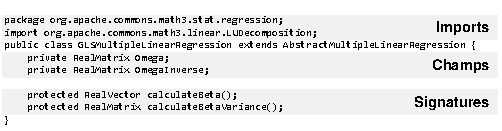
\includegraphics[width=0.92\textwidth]{assets/coderujb-figure2a-context-fr.pdf}\par}
{\scriptsize Fig. 2(a), extrait adapté : annotations traduites ; ce n’est pas le prompt complet.\par}
\medskip
\begin{columns}[c,onlytextwidth]
\begin{column}{0.38\textwidth}
\textbf{CodeLlama-13B}\par
\smallskip
Génération de fonctions (FCG)\par
\medskip
Trois prompts, un même modèle.
\end{column}
\begin{column}{0.59\textwidth}
\centering
\renewcommand{\arraystretch}{1.2}
\begin{tabular}{@{}lr@{}}
\toprule
\textbf{Prompt} & \textbf{pass-all@1} \\
\midrule
Un exemple & 12,84 \% \\
Quatre exemples & 14,50 \% \\
Contexte du projet & 21,91 \% \\
\bottomrule
\end{tabular}
\end{column}
\end{columns}
\medskip
{\scriptsize Source : Zeng et al., ISSTA 2024, fig. 2(a) et tableau 3.\par}

\note{
INTERVENANT 3 — Jianye SHI — Résultats : contexte et modèles

DIAPOSITIVE 14 / 32

Merci Hao. Après la méthode, passons aux résultats. Première question : quelles informations faut-il fournir au modèle pour générer une fonction ? En haut de la diapositive, on voit le contexte extrait de la classe : les imports, les champs et les signatures des autres méthodes.

Sur le tableau, avec CodeLlama-13B, donner un ou quatre exemples change peu le score : on reste entre 13 et 14,5 \%. En revanche, avec le contexte du projet, on grimpe à près de 22 \%. Connaître la structure de la classe aide donc bien plus que d'ajouter des exemples.

REPÈRES : RQ1 / contexte du projet / exemples

SOURCE : Zeng et al. (2024), CoderUJB: An Executable and Unified Java Benchmark for Practical Programming Scenarios. §3.4, figure 2(a) et RQ1, tableau 3, pp. 128, 131. DOI: 10.1145/3650212.3652115.

Les chiffres de ces diapositives proviennent de l’article. Partie 3 : environ 374 mots ; durée à vérifier par répétition chronométrée.
}
\end{frame}

% Slide 15 / 32; intervenant 3

\begin{frame}{Un écart plus marqué en réparation}
\small
FCG : générer une fonction \hfill APR : réparer une fonction
\medskip
\begin{center}
\normalsize
\renewcommand{\arraystretch}{1.65}
\begin{tabular}{@{}l@{\hspace{10mm}}r@{\hspace{10mm}}r@{}}
\toprule
\textbf{Modèle} & \textbf{FCG} & \textbf{APR} \\
\midrule
CodeLlama-34B & 22,82 \% & 5,01 \% \\
GPT-3.5-Turbo & 23,37 \% & 9,31 \% \\
\textbf{GPT-4} & \textbf{30,52 \%} & \textbf{18,76 \%} \\
\bottomrule
\end{tabular}
\end{center}
\medskip
Écart GPT-4 / CodeLlama : \textbf{7,70 points} en FCG, \textbf{13,75} en APR.\par
\medskip
{\scriptsize pass-all@1. Source : Zeng et al., tableau 4.\par
Versions : GPT-3.5-Turbo-0301 et GPT-4-0314.\par}

\note{
INTERVENANT 3 — Jianye SHI — Résultats : contexte et modèles

DIAPOSITIVE 15 / 32

Voyons maintenant comment les modèles se comparent dans le tableau 4, en prenant CodeLlama-34B face à GPT-3.5 et GPT-4.

En génération de fonctions, CodeLlama fait jeu égal avec GPT-3.5 autour de 23 \%, contre 30,5 \% pour GPT-4. Mais en réparation de bugs, tous les scores chutent et l’écart se creuse : CodeLlama tombe à 5 \%, contre 9 \% pour GPT-3.5 et près de 19 \% pour GPT-4. L’écart avec GPT-4 passe ainsi de 8 à près de 14 points.

REPÈRES : RQ2 / mêmes métriques / modèles de l’étude

SOURCE : Zeng et al. (2024), CoderUJB: An Executable and Unified Java Benchmark for Practical Programming Scenarios. Tableaux 2 et 4, pp. 130, 132. DOI: 10.1145/3650212.3652115.

Les chiffres de ces diapositives proviennent de l’article. Le tableau concerne GPT-3.5-Turbo-0301 et GPT-4-0314. Partie 3 : environ 374 mots ; durée à vérifier par répétition chronométrée.
}
\end{frame}

% Slide 16 / 32; intervenant 3

\begin{frame}{GPT-4 : des scores différents selon la tâche}
\small
\textbf{GPT-4-0314} \hfill pass-all@1 (\%)
\medskip
\begin{center}
\begin{tikzpicture}[x=0.17cm,y=0.72cm]
\foreach \x in {0,10,20,30} {
  \draw[black!15] (\x,-0.45) -- (\x,3.45);
  \node[font=\scriptsize,anchor=north] at (\x,-0.5) {\x};
}
\foreach \y/\v/\label/\val in {3/30.52/{FCG : générer}/30{,}52,2/24.18/{CTG : tester le code}/24{,}18,1/6.66/{ITG : reproduire un bug}/6{,}66,0/18.76/{APR : réparer}/18{,}76} {
  \fill[structure.fg] (0,\y-0.17) rectangle (\v,\y+0.17);
  \node[anchor=east,font=\small] at (-1,\y) {\label};
  \node[anchor=west,font=\small] at (\v+0.5,\y) {\val\,\%};
}
\end{tikzpicture}
\end{center}
\smallskip
{\footnotesize
\textbf{Réussite :} FCG / APR : passer les tests.\par
CTG : test exécutable couvrant le code.\par
ITG : test en échec avec le bug, puis réussi après correction.\par}
\smallskip
{\scriptsize Source : Zeng et al., §3.5 et tableau 4.\par}

\note{
INTERVENANT 3 — Jianye SHI — Résultats : contexte et modèles

DIAPOSITIVE 16 / 32

Même pour GPT-4, les résultats varient fortement selon la tâche. S'il dépasse 30 \% en génération et 24 \% pour tester le code, il descend à 19 \% en réparation, et chute à 6,66 \% en ITG pour reproduire un bug.

Pour lire ces scores, il faut aussi tenir compte des critères de réussite. En FCG et APR, il faut passer les tests existants ; en CTG, le test doit s’exécuter et couvrir le code. Mais en ITG, le modèle part du rapport de bug, sans le contexte de classe : son test doit échouer sur la version défectueuse, puis réussir après correction.

REPÈRES : FCG / CTG / ITG / APR

SOURCE : Zeng et al. (2024), CoderUJB: An Executable and Unified Java Benchmark for Practical Programming Scenarios. Tableau 4, p. 132 ; valeurs choisies plutôt que le texte contradictoire de RQ2. DOI: 10.1145/3650212.3652115.

Les chiffres de ces diapositives proviennent de l’article. Le tableau concerne GPT-3.5-Turbo-0301 et GPT-4-0314. Partie 3 : environ 374 mots ; durée à vérifier par répétition chronométrée.
}
\end{frame}

% Slide 17 / 32; intervenant 3

\begin{frame}{Détecter les bugs reste difficile}
\small
\begin{center}
\renewcommand{\arraystretch}{1.8}
\begin{tabular}{@{}>{\centering\arraybackslash}p{0.28\textwidth}>{\centering\arraybackslash}p{0.32\textwidth}>{\centering\arraybackslash}p{0.30\textwidth}@{}}
{\LARGE\structure{940}} & {\LARGE\structure{50\,\%}} & {\LARGE\structure{52,16\,\%}} \\
fonctions & réponse constante & GPT-4 \\
\end{tabular}
\end{center}
\medskip
470 fonctions avec un bug et 470 versions corrigées.\par
\smallskip
\textbf{Accuracy :} proportion de réponses correctes.\par
GPT-4 dépasse la référence de \textbf{2,16 points}.
\bigskip
\begin{block}{À retenir}
Le contexte aide la génération. Les autres tâches restent à vérifier séparément.
\end{block}
\smallskip
{\scriptsize Source : Zeng et al., §3.3 et tableau 4 ; GPT-4-0314.\par}

\note{
INTERVENANT 3 — Jianye SHI — Résultats : contexte et modèles

DIAPOSITIVE 17 / 32

Enfin, même détecter un bug reste très difficile. Sur les 940 fonctions — 470 avec bug et 470 corrigées — répondre toujours la même chose donne déjà 50 \%.

Or, GPT-4 atteint seulement 52,16 \% d’accuracy, à peine deux points au-dessus de cette référence. Les auteurs l'expliquent par la complexité des erreurs logiques dans de vrais projets.

En résumé, le contexte aide à générer une fonction, mais cela ne garantit pas de savoir réparer ou détecter un bug. L’entraînement spécialisé ou l'instruction tuning permettent-ils de faire mieux ? Je laisse la parole à Xiang.

REPÈRES : 940 exemples / 50 \% / 52,16 \%

SOURCE : Zeng et al. (2024), CoderUJB: An Executable and Unified Java Benchmark for Practical Programming Scenarios. §3.3, RQ2 et tableau 4, pp. 128, 132. DOI: 10.1145/3650212.3652115.

Les chiffres de ces diapositives proviennent de l’article. Le tableau concerne GPT-3.5-Turbo-0301 et GPT-4-0314. Partie 3 : environ 374 mots ; durée à vérifier par répétition chronométrée.
}
\end{frame}

\section{Résultats : effets de l’entraînement}

% Slide 19 / 32; intervenant 4

\begin{frame}{Plus d’entraînement = de meilleures performances ?}
\small
\begin{block}{RQ3 : préentraînement spécialisé par langage}
\begin{itemize}
  \item Continuer l’entraînement avec du code Python ou Java
\end{itemize}
\end{block}
\begin{block}{RQ4 : ajustement sur instructions}
\begin{itemize}
  \item Apprendre à suivre des demandes grâce à des exemples de réponses
\end{itemize}
\end{block}
\medskip
{\small Question commune : quel effet sur les tâches réelles de CoderUJB ?\par}

\note{
INTERVENANT 4 — Xiang BIAN — Résultats : effets de l’entraînement

DIAPOSITIVE 19 / 32

Je vais maintenant expliquer les effets de deux types d’entraînement. 

Le premier est le préentraînement supplémentaire dans un langage précis. Par exemple, on continue à entraîner le modèle avec du code Python ou Java.

Le second est l’ajustement sur des instructions. On entraîne alors le modèle à répondre à des demandes avec des exemples de tâches et de réponses.

Ils comparent ces versions aux modèles de départ : quelles tâches progressent ?

REPÈRES : RQ3 / continued pre-training / RQ4 / instruction tuning

SOURCE : Zeng et al. (2024), CoderUJB: An Executable and Unified Java Benchmark for Practical Programming Scenarios. §4.1-4.2, RQ3-RQ4, pp. 130, 133. DOI: 10.1145/3650212.3652115.

Les chiffres reprennent l'article et n'ont pas été reproduits par notre groupe. Le temps de présentation de cette partie mise à jour est à vérifier par répétition chronométrée.
}
\end{frame}

% Slide 20 / 32; intervenant 4

\begin{frame}{Se spécialiser dans un langage : un compromis}
\small
\textbf{StarCoder-15B}
\medskip

\begin{columns}[T,onlytextwidth]
\begin{column}{0.49\textwidth}
\textbf{CoderUJB FCG / Java}
\medskip

\renewcommand{\arraystretch}{1.65}
\begin{tabular}{@{}l@{\quad}l@{\quad}r@{}}
Base & \makebox[2.6cm][l]{\textcolor{structure.fg}{\rule{0.9958cm}{1.1ex}}} & 15,32 \% \\
+ Python & \makebox[2.6cm][l]{\textcolor{structure.fg}{\rule{0.9354cm}{1.1ex}}} & 14,39 \% \\
+ Java & \makebox[2.6cm][l]{\textcolor{structure.fg}{\rule{1.2233cm}{1.1ex}}} & 18,82 \% \\
\end{tabular}
\end{column}
\begin{column}{0.49\textwidth}
\textbf{HumanEval / Python}
\medskip

\renewcommand{\arraystretch}{1.65}
\begin{tabular}{@{}l@{\quad}l@{\quad}r@{}}
Base & \makebox[2.6cm][l]{\textcolor{structure.fg}{\rule{1.9728cm}{1.1ex}}} & 30,35 \% \\
+ Python & \makebox[2.6cm][l]{\textcolor{structure.fg}{\rule{2.1821cm}{1.1ex}}} & 33,57 \% \\
+ Java & \makebox[2.6cm][l]{\textcolor{structure.fg}{\rule{1.7596cm}{1.1ex}}} & 27,07 \% \\
\end{tabular}
\end{column}
\end{columns}
\bigskip
\textbf{En FCG, la spécialisation favorise généralement le langage ciblé.}
\medskip

{\small Mais ce résultat n’est pas systématique pour ITG et APR (RQ3).\par}

\note{
INTERVENANT 4 — Xiang BIAN — Résultats : effets de l’entraînement

DIAPOSITIVE 20 / 32

Voici un exemple avec StarCoder. Sur la génération de fonctions Java de CoderUJB, le modèle de base obtient environ quinze pour cent. La version entraînée davantage sur Python descend à environ quatorze pour cent. La version Java monte à environ dix-neuf pour cent.

Sur HumanEval en Python, on observe le mouvement inverse : la version Python progresse et la version Java recule.

Cela illustre un compromis entre langages. Mais pour reproduire des bugs ou réparer des fonctions, les auteurs observent des effets moins réguliers. Il ne faut donc pas généraliser cet exemple à toutes les tâches.

REPÈRES : StarCoder-15B / FCG / pass-all@1 / RQ3

SOURCE : Zeng et al. (2024), CoderUJB: An Executable and Unified Java Benchmark for Practical Programming Scenarios. RQ3 et tableau 4, pp. 132-133. DOI: 10.1145/3650212.3652115.

Les chiffres reprennent l'article et n'ont pas été reproduits par notre groupe. Le temps de présentation de cette partie mise à jour est à vérifier par répétition chronométrée.
}
\end{frame}

% Slide 21 / 32; intervenant 4

\begin{frame}{L’instruction tuning n’améliore pas toutes les tâches}
\small
\textbf{CodeLlama-13B}
\begin{center}
\renewcommand{\arraystretch}{1.15}
\begin{tabular}{@{}lrr@{}}
\toprule
\textbf{Tâche et indicateur} & \textbf{Base} & \textbf{Instruct} \\
\midrule
FCG : pass-all@1 & 21,91 \% & 13,28 \% \\
CTG : pass-all@1 & 12,61 \% & 6,14 \% \\
APR : pass-all@1 & 4,50 \% & 4,09 \% \\
APR : pass-all@10 & 8,39 \% & 15,72 \% \\
\bottomrule
\end{tabular}
\end{center}
\smallskip
\textbf{Tableau 5 : pourquoi la génération se dégrade-t-elle ?}

{\footnotesize FCG, CodeLlama-13B\par}
\begin{center}
\renewcommand{\arraystretch}{1.1}
\begin{tabular}{@{}lrr@{}}
\toprule
\textbf{Indicateur} & \textbf{Base} & \textbf{Instruct} \\
\midrule
Syntaxe & 94,14 \% & 95,99 \% \\
Compilation & 63,49 \% & 40,76 \% \\
\bottomrule
\end{tabular}
\end{center}
{\small La syntaxe reste correcte, mais le code compile moins souvent.\par}

\note{
INTERVENANT 4 — Xiang BIAN — Résultats : effets de l’entraînement

DIAPOSITIVE 21 / 32

L’ajustement sur instructions donne aussi des résultats contrastés. Regardons CodeLlama treize milliards et sa version Instruct.

Pour compléter une fonction, le score à une tentative passe d’environ vingt-deux à treize pour cent. Pour créer un test à partir du code, il passe d’environ treize à six pour cent.

Pour la réparation, il faut préciser le nombre de tentatives. Avec une seule proposition, le score baisse légèrement. Avec dix propositions, il passe d’environ huit à seize pour cent.

Le tableau cinq donne un autre élément. Pour cette même tâche de génération de fonctions, la syntaxe reste presque aussi bonne : environ quatre-vingt-quatorze pour cent pour le modèle de base et quatre-vingt-seize pour cent pour Instruct. Mais le taux de compilation passe d’environ soixante-trois à quarante et un pour cent. Une syntaxe correcte ne suffit donc pas pour compiler dans le projet.

Dire simplement que les instructions améliorent la réparation serait donc trop général. La métrique compte aussi.

REPÈRES : CodeLlama-13B / pass-all@k / syntaxe / compilation

SOURCE : Zeng et al. (2024), CoderUJB: An Executable and Unified Java Benchmark for Practical Programming Scenarios. RQ4 et tableaux 4-5, pp. 132-134. DOI: 10.1145/3650212.3652115.

Les chiffres reprennent l'article et n'ont pas été reproduits par notre groupe. Le temps de présentation de cette partie mise à jour est à vérifier par répétition chronométrée.
}
\end{frame}

% Slide 22 / 32; intervenant 4

\begin{frame}{Plus d’entraînement $\ne$ meilleures performances}
\small
\begin{block}{RQ3 : préentraînement par langage}
La spécialisation aide certaines tâches, mais ses effets varient selon le langage et la tâche.
\end{block}
\begin{block}{RQ4 : instruction fine-tuning}
La génération peut se dégrader ; certaines réparations peuvent s’améliorer.
\end{block}
\begin{block}{Interprétation des auteurs}
La proximité entre préentraînement et tâche évaluée pourrait expliquer ces différences.
\end{block}
\medskip
{\small Cas particulier : CodeLlama-Instruct-34B produit des réponses répétées (mode collapse).\par}

\note{
INTERVENANT 4 — Xiang BIAN — Résultats : effets de l’entraînement

DIAPOSITIVE 22 / 32

Les auteurs proposent une explication : l’effet de l’entraînement pourrait dépendre de la proximité entre la tâche évaluée et la tâche de préentraînement. C’est une interprétation des résultats, pas une règle démontrée pour tous les modèles.

CodeLlama Instruct trente-quatre milliards produit des réponses identiques pour différentes questions dans certaines tâches. Les auteurs parlent d’un effondrement du mode de génération et écartent ces résultats de leur analyse correspondante.

Nous retenons donc qu’il faut tester chaque stratégie sur plusieurs tâches. La personne suivante va préciser les limites de cette étude.

REPÈRES : RQ3 / RQ4 / effets selon la tâche / prudence

SOURCE : Zeng et al. (2024), CoderUJB: An Executable and Unified Java Benchmark for Practical Programming Scenarios. RQ3-RQ4, tableau 5 et discussion, pp. 133-134. DOI: 10.1145/3650212.3652115.

Les chiffres reprennent l'article et n'ont pas été reproduits par notre groupe. Le temps de présentation de cette partie mise à jour est à vérifier par répétition chronométrée.
}
\end{frame}

\section{Limites de l’étude}

% Slide 24 / 32; intervenant 5

\begin{frame}{Les trois limites principales}
\small
\begin{block}{Validité interne}
\begin{itemize}
  \item Erreurs possibles dans les scripts
\end{itemize}
\end{block}
\begin{block}{Validité externe}
\begin{itemize}
  \item Choix des modèles et généralisation
\end{itemize}
\end{block}
\begin{block}{Validité des mesures}
\begin{itemize}
  \item Indicateurs et qualité des tests
\end{itemize}
\end{block}
\medskip
{\small Les auteurs cherchent à limiter ces risques.\par}

\note{
INTERVENANT 5 — Zijie Fang — Limites de l’étude

DIAPOSITIVE 24 / 32

Je vais maintenant présenter les limites de l’étude. Je distingue celles que les auteurs discutent explicitement et les réserves que nous ajoutons.

Dans leur section sur la validité, les auteurs présentent trois types de risques. Le premier concerne les erreurs possibles dans les scripts. Le deuxième concerne le choix des modèles et la portée des conclusions. Le troisième concerne les indicateurs utilisés.

Les auteurs cherchent à réduire ces risques, sans pouvoir les supprimer.

REPÈRES : validité interne / externe / des mesures

SOURCE : Zeng et al. (2024), CoderUJB: An Executable and Unified Java Benchmark for Practical Programming Scenarios. §6, p. 134. DOI: 10.1145/3650212.3652115.

Les chiffres reprennent l'article et n'ont pas été reproduits par notre groupe. Partie 5 : 346 mots ; cible inférieure à 4 minutes, à vérifier par répétition chronométrée.
}
\end{frame}

% Slide 25 / 32; intervenant 5

\begin{frame}{Réussir les tests ne suffit pas}
\small
\begin{block}{Ce que font les auteurs}
\begin{itemize}
  \item Vérification des scripts et publication des résultats
\end{itemize}
\end{block}
\begin{block}{Limite des tests}
\begin{itemize}
  \item Un programme peut encore contenir des bugs
\end{itemize}
\end{block}
\begin{block}{Limite de la couverture}
\begin{itemize}
  \item Exécuter du code $\ne$ vérifier tous ses comportements
\end{itemize}
\end{block}
\medskip
{\small Passer les tests $\ne$ correction garantie.\par}

\note{
INTERVENANT 5 — Zijie Fang — Limites de l’étude

DIAPOSITIVE 25 / 32

Pour les erreurs d’implémentation, les auteurs expliquent qu’ils ont relu leurs scripts. Ils publient également le code et les résultats pour permettre des vérifications.

Concernant les mesures, ils utilisent plusieurs indicateurs et vérifient la couverture des tests. C’est utile, mais un programme qui passe les tests peut encore contenir un bug non détecté.

De même, couvrir une ligne signifie qu’un test l’a exécutée. Cela ne garantit pas que le test vérifie correctement tous les comportements. Il faut donc comprendre les scores comme une réussite selon les critères du benchmark, pas comme une preuve de correction totale.

REPÈRES : code public / tests / couverture

SOURCE : Zeng et al. (2024), CoderUJB: An Executable and Unified Java Benchmark for Practical Programming Scenarios. §3.5 et §6, pp. 129-130, 134 ; distinction couverture/correction : analyse du groupe. DOI: 10.1145/3650212.3652115.

Les chiffres reprennent l'article et n'ont pas été reproduits par notre groupe. Partie 5 : 346 mots ; cible inférieure à 4 minutes, à vérifier par répétition chronométrée.
}
\end{frame}

% Slide 26 / 32; intervenant 5

\begin{frame}{Des résultats difficiles à généraliser}
\small
\begin{block}{Modèles}
\begin{itemize}
  \item Des versions précises des LLM
\end{itemize}
\end{block}
\begin{block}{Données}
\begin{itemize}
  \item 17 projets Java issus de Defects4J
\end{itemize}
\end{block}
\begin{block}{Réparation (APR)}
\begin{itemize}
  \item Des bugs dans une seule fonction
\end{itemize}
\end{block}
\medskip
{\small Pas être généralisés à tous les cas.\par}

\note{
INTERVENANT 5 — Zijie Fang — Limites de l’étude

DIAPOSITIVE 26 / 32

Les auteurs choisissent des modèles qu’ils considèrent comme représentatifs. Mais ce sont des versions précises, évaluées dans les conditions de cette étude.

Nous ajoutons une réserve sur les données. Les questions proviennent de dix-sept projets Java d’une même source. Cela facilite une construction cohérente, mais ne représente pas tous les langages ni tous les logiciels.

De plus, la réparation se concentre sur des défauts dans une seule fonction. On ne peut donc pas supposer que les résultats seraient identiques pour une correction répartie dans plusieurs fichiers.

REPÈRES : Java / 17 projets / versions testées

SOURCE : Zeng et al. (2024), CoderUJB: An Executable and Unified Java Benchmark for Practical Programming Scenarios. §3.2-3.3, §4.2, §6, pp. 127-130, 134 ; portée des projets : analyse du groupe. DOI: 10.1145/3650212.3652115.

Les chiffres reprennent l'article et n'ont pas été reproduits par notre groupe. Partie 5 : 346 mots ; cible inférieure à 4 minutes, à vérifier par répétition chronométrée.
}
\end{frame}

% Slide 27 / 32; intervenant 5

\begin{frame}{Une évaluation encore limitée}
\small
\begin{block}{Protocole étudié}
\begin{itemize}
  \item Prompt $\rightarrow$ réponse $\rightarrow$ évaluation
\end{itemize}
\end{block}
\begin{block}{Autre approche possible}
\begin{itemize}
  \item Tester $\rightarrow$ corriger $\rightarrow$ recommencer
\end{itemize}
\end{block}
\begin{block}{Contexte fourni}
\begin{itemize}
  \item Le modèle ne reçoit pas forcément tout le projet
\end{itemize}
\end{block}
\medskip
{\small Ces limites précisent la portée des conclusions.\par}

\note{
INTERVENANT 5 — Zijie Fang — Limites de l’étude

DIAPOSITIVE 27 / 32

Enfin, les auteurs étudient principalement des réponses à des questions ou des complétions de code. Ils ne mesurent pas toute l’activité d’un développeur assisté par une IA.

Par exemple, une méthode qui exécute ses propres tests puis corrige plusieurs fois sa réponse pourrait se comporter autrement. 

Il faut aussi distinguer le projet disponible dans le benchmark et le contexte réellement fourni au modèle. Une information absente du prompt peut influencer le résultat.

Ces limites précisent donc où les conclusions s’appliquent. La dernière partie va proposer notre évaluation et des améliorations possibles.

REPÈRES : prompt / réponse / outils / portée

SOURCE : Zeng et al. (2024), CoderUJB: An Executable and Unified Java Benchmark for Practical Programming Scenarios. §3.4 et conclusion 2 de RQ2, pp. 128-129, 132 ; portée du protocole : analyse du groupe. DOI: 10.1145/3650212.3652115.

Les chiffres reprennent l'article et n'ont pas été reproduits par notre groupe. Partie 5 : 346 mots ; cible inférieure à 4 minutes, à vérifier par répétition chronométrée.
}
\end{frame}

\section{Critique et conclusion}

% Slide 29 / 32; intervenant 6

\begin{frame}{Notre évaluation : un apport utile}
\small
\begin{block}{Pertinence}
\begin{itemize}
  \item Plusieurs activités réelles de développement
\end{itemize}
\end{block}
\begin{block}{Vérification}
\begin{itemize}
  \item Exécution et critères adaptés aux tâches
\end{itemize}
\end{block}
\begin{block}{Transparence}
\begin{itemize}
  \item Code, scripts et résultats rendus publics
\end{itemize}
\end{block}
\medskip
{\small Notre appréciation : une contribution à la méthode d’évaluation, au-delà d’un classement.\par}

\note{
INTERVENANT 6 — Yupan Huang — Critique et conclusion

DIAPOSITIVE 29 / 32

Pour terminer, voici notre évaluation de l’article. Son principal point fort est de rapprocher l’évaluation de plusieurs activités réelles de développement.

Les auteurs réunissent plusieurs tâches, utilisent des projets existants et vérifient les solutions avec des critères adaptés. Ils rendent aussi leurs données et leurs résultats accessibles. 

Nous apprécions surtout le fait de regarder les résultats par tâche. Un seul score peut masquer des différences importantes. Cet apport concerne aussi la manière d’évaluer les futurs modèles.

REPÈRES : forces / tâches / exécution / transparence

SOURCE : Zeng et al. (2024), CoderUJB: An Executable and Unified Java Benchmark for Practical Programming Scenarios. §3, §5-7, pp. 126-130, 134 ; appréciation du groupe. DOI: 10.1145/3650212.3652115.

Les chiffres reprennent l'article et n'ont pas été reproduits par notre groupe. Partie 6 : 348 mots ; cible inférieure à 4 minutes, à vérifier par répétition chronométrée.
}
\end{frame}

% Slide 30 / 32; intervenant 6

\begin{frame}{Des comparaisons à mieux isoler}
\small
\begin{block}{Constat du protocole}
\begin{itemize}
  \item Base : complétion ; Instruct : dialogue
\end{itemize}
\end{block}
\begin{block}{Réserve}
\begin{itemize}
  \item Le format peut contribuer à l’écart observé
\end{itemize}
\end{block}
\begin{block}{Amélioration proposée}
\begin{itemize}
  \item Tester plusieurs formats et quantifier l’incertitude
\end{itemize}
\end{block}
\medskip
{\small Un contenu équivalent ne garantit pas un effet identique du format.\par}

\note{
INTERVENANT 6 — Yupan Huang — Critique et conclusion

DIAPOSITIVE 30 / 32

Notre première réserve concerne l’interprétation des différences entre modèles. Les modèles de base utilisent un format de complétion. Les modèles ajustés sur instructions utilisent un format de dialogue.

Les auteurs gardent le même contenu et considèrent ces formats comme équivalents. Mais le format peut aussi influencer la réponse. Nous voudrions donc une expérience supplémentaire qui sépare mieux l’effet de l’entraînement et celui du prompt.

Nous proposerions aussi plusieurs répétitions et des intervalles d’incertitude. Ce sont nos propositions pour vérifier la stabilité des écarts.

REPÈRES : format du prompt / entraînement / protocole

SOURCE : Zeng et al. (2024), CoderUJB: An Executable and Unified Java Benchmark for Practical Programming Scenarios. §3.4, §4.2, pp. 128, 130 ; critique et propositions du groupe. DOI: 10.1145/3650212.3652115.

Les chiffres reprennent l'article et n'ont pas été reproduits par notre groupe. Partie 6 : 348 mots ; cible inférieure à 4 minutes, à vérifier par répétition chronométrée.
}
\end{frame}

% Slide 31 / 32; intervenant 6

\begin{frame}{Une lecture attentive des chiffres}
\small
\textbf{GPT-4, tâche ITG}
\begin{center}
\small
\renewcommand{\arraystretch}{1.35}
\begin{tabular}{@{}lr@{}}
\toprule
\textbf{Indicateur} & \textbf{Valeur du tableau 4} \\
\midrule
pass-all@1 & 6,66 \% \\
pass-all@10 & 15,76 \% \\
\bottomrule
\end{tabular}
\end{center}
\medskip
{\small RQ2 mentionne 15,76 parmi des scores annoncés à k = 1. Nos diapositives suivent le tableau 4.\par}

\note{
INTERVENANT 6 — Yupan Huang — Critique et conclusion

DIAPOSITIVE 31 / 32

Autre remarque : certains chiffres sont incohérents. Pour GPT quatre, le tableau quatre donne six virgule soixante-six pour cent en génération de tests à partir d’un bug, avec une tentative.

Le texte du résultat deux mentionne quinze virgule soixante-seize pour cent dans une liste présentée comme des scores à une tentative. Or ce chiffre correspond à dix tentatives dans le tableau.

Nous avons donc utilisé les valeurs du tableau et indiqué k sur nos diapositives. Cette incohérence mérite une correction, mais elle ne suffit pas, à elle seule, à invalider l’ensemble de l’étude.

REPÈRES : tableau 4 / k = 1 / k = 10

SOURCE : Zeng et al. (2024), CoderUJB: An Executable and Unified Java Benchmark for Practical Programming Scenarios. RQ2, p. 131 et tableau 4, p. 132 ; incohérence vérifiée par le groupe. DOI: 10.1145/3650212.3652115.

Les chiffres reprennent l'article et n'ont pas été reproduits par notre groupe. Partie 6 : 348 mots ; cible inférieure à 4 minutes, à vérifier par répétition chronométrée.
}
\end{frame}

% Slide 32 / 32; intervenant 6

\begin{frame}{Conclusion et pistes de prolongement}
\small
\begin{block}{Élargir}
\begin{itemize}
  \item Autres projets, langages et méthodes avec outils
\end{itemize}
\end{block}
\begin{block}{Contrôler}
\begin{itemize}
  \item Risque de contamination et sensibilité au protocole
\end{itemize}
\end{block}
\begin{block}{Retenir}
\begin{itemize}
  \item Comparer par tâche, avec la même métrique
\end{itemize}
\end{block}
\medskip
{\small CoderUJB : une base utile pour une évaluation plus réaliste, dans un périmètre défini.\par}

\note{
INTERVENANT 6 — Yupan Huang — Critique et conclusion

DIAPOSITIVE 32 / 32

Pour prolonger cette étude, nous proposerions des projets plus variés, d’autres langages et une vérification du risque de présence des exemples dans les données d’entraînement. Nous testerions aussi des méthodes capables d’utiliser des outils et de corriger leurs réponses.

En conclusion, CoderUJB montre l’intérêt d’évaluer les modèles dans un contexte de projet et sur plusieurs tâches. Les effets de l’entraînement varient, et les indicateurs doivent être lus avec précision.

Notre bilan est donc positif, avec des réserves sur la portée et sur certaines comparaisons. Merci pour votre attention. Nous sommes prêts à répondre à vos questions.

REPÈRES : plus de diversité / contrôles / évaluation par tâche

SOURCE : Zeng et al. (2024), CoderUJB: An Executable and Unified Java Benchmark for Practical Programming Scenarios. §5-7, p. 134 ; prolongements et bilan du groupe. DOI: 10.1145/3650212.3652115.

Les chiffres reprennent l'article et n'ont pas été reproduits par notre groupe. Partie 6 : 348 mots ; cible inférieure à 4 minutes, à vérifier par répétition chronométrée.
}
\end{frame}

\end{document}
